\begin{figure}[t]
\centering
\resizebox{\columnwidth}{!}{%
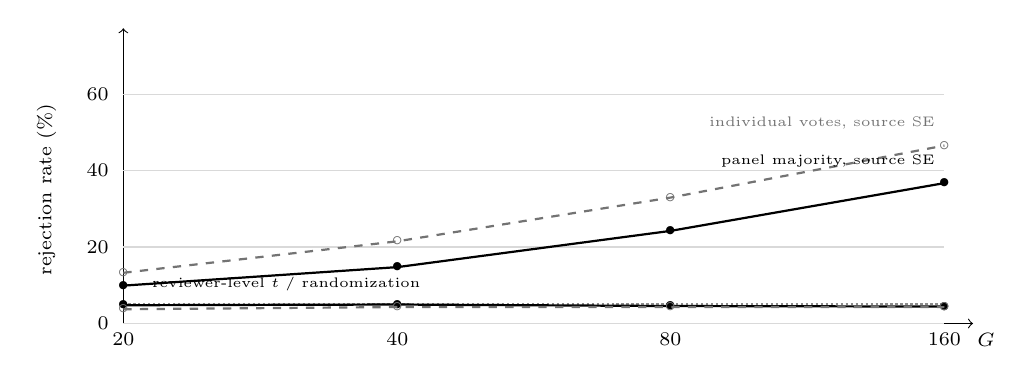
\begin{tikzpicture}[font=\scriptsize]
\draw[->] (0,0) -- (0.89\columnwidth,0) node[right, xshift=-2pt, yshift=-6pt] {$G$};
\draw[->] (0,0) -- (0,3.75cm);
\node[rotate=90, anchor=south] at (-0.06\columnwidth,1.70cm) {rejection rate (\%)};
\draw[black!15] (0,0.000cm) -- (0.86\columnwidth,0.000cm);
\node[anchor=east] at (-0.005\columnwidth,0.000cm) {0};
\draw[black!15] (0,0.971cm) -- (0.86\columnwidth,0.971cm);
\node[anchor=east] at (-0.005\columnwidth,0.971cm) {20};
\draw[black!15] (0,1.943cm) -- (0.86\columnwidth,1.943cm);
\node[anchor=east] at (-0.005\columnwidth,1.943cm) {40};
\draw[black!15] (0,2.914cm) -- (0.86\columnwidth,2.914cm);
\node[anchor=east] at (-0.005\columnwidth,2.914cm) {60};
\draw[black!45, densely dotted, thick] (0,0.243cm) -- (0.86\columnwidth,0.243cm);
\node[anchor=north] at (0.000\columnwidth,0) {20};
\node[anchor=north] at (0.287\columnwidth,0) {40};
\node[anchor=north] at (0.573\columnwidth,0) {80};
\node[anchor=north] at (0.860\columnwidth,0) {160};
\draw[black, solid, thick] (0.000\columnwidth,0.481cm) -- (0.287\columnwidth,0.716cm) -- (0.573\columnwidth,1.176cm) -- (0.860\columnwidth,1.783cm);
\node[black] at (0.000\columnwidth,0.481cm) {$\bullet$};
\node[black] at (0.287\columnwidth,0.716cm) {$\bullet$};
\node[black] at (0.573\columnwidth,1.176cm) {$\bullet$};
\node[black] at (0.860\columnwidth,1.783cm) {$\bullet$};
\draw[black!55, dashed, thick] (0.000\columnwidth,0.644cm) -- (0.287\columnwidth,1.044cm) -- (0.573\columnwidth,1.599cm) -- (0.860\columnwidth,2.260cm);
\node[black!55] at (0.000\columnwidth,0.644cm) {$\circ$};
\node[black!55] at (0.287\columnwidth,1.044cm) {$\circ$};
\node[black!55] at (0.573\columnwidth,1.599cm) {$\circ$};
\node[black!55] at (0.860\columnwidth,2.260cm) {$\circ$};
\draw[black, solid, thick] (0.000\columnwidth,0.232cm) -- (0.287\columnwidth,0.241cm) -- (0.573\columnwidth,0.222cm) -- (0.860\columnwidth,0.215cm);
\node[black] at (0.000\columnwidth,0.232cm) {$\bullet$};
\node[black] at (0.287\columnwidth,0.241cm) {$\bullet$};
\node[black] at (0.573\columnwidth,0.222cm) {$\bullet$};
\node[black] at (0.860\columnwidth,0.215cm) {$\bullet$};
\draw[black!55, dashed, thick] (0.000\columnwidth,0.181cm) -- (0.287\columnwidth,0.209cm) -- (0.573\columnwidth,0.210cm) -- (0.860\columnwidth,0.208cm);
\node[black!55] at (0.000\columnwidth,0.181cm) {$\circ$};
\node[black!55] at (0.287\columnwidth,0.209cm) {$\circ$};
\node[black!55] at (0.573\columnwidth,0.210cm) {$\circ$};
\node[black!55] at (0.860\columnwidth,0.208cm) {$\circ$};
\node[anchor=east, font=\tiny] at (0.86\columnwidth,2.06cm) {panel majority, source SE};
\node[anchor=east, font=\tiny, black!55] at (0.86\columnwidth,2.54cm) {individual votes, source SE};
\node[anchor=west, font=\tiny] at (0.02\columnwidth,0.50cm) {reviewer-level $t$ / randomization};
\end{tikzpicture}}
\caption{Null rejection rate against the number of sources $G$ at the estimated reviewer heterogeneity $\sigma_r=0.27$, with reviewer abilities redrawn each replicate. Adding sources makes the two source-level analyses steadily worse, and using individual votes instead of majority labels does not help: the defect is the unit of uncertainty, not the aggregation. The two reviewer-level analyses stay at the nominal level and are executable from released pre-aggregation votes. Table~\ref{tab:retrospective-remedies} gives the values and the corresponding power.}
\label{fig:remedy-calibration}
\end{figure}
